\documentclass[a4paper,12pt]{article}
%%% acentos en LaTeX
\usepackage[utf8]{inputenc}
\usepackage[spanish]{babel}

% Figures within a column...
\makeatletter
\newenvironment{tablehere}
{\def\@captype{table}}
{}
\newenvironment{figurehere}
{\def\@captype{figure}}
{}
\makeatother

\title{ \Huge Universidad Veracruzana\\[1in]
		\Huge Termodinámica de sistemas abiertos}
\author{Carlos Manuel Rodríguez y Martínez}
\date{21/05/2012}
 
\usepackage{graphicx}
\usepackage{amsmath}
\usepackage{amssymb}


\usepackage{multicol}
\usepackage{hyperref}
\usepackage{amsfonts}

\begin{document}
\maketitle
\newpage

\tableofcontents

\section{Introducción}
Si bien la termodinámica desarrollada hasta ahora es aplicable únicamente a sistemas cerrados raramente se encuentra un sistema termodinámico en la naturaleza que corresponda a a este tipo de descripción. La razón de esto es que un sistema termodinámico real nunca es capaz de lograr un aislamiento tal que no exista el intercambio de masa con sus alrededores, aunque es cierto que se puede disminuir este efecto hasta llegar a límites descriptibles con la termodinámica de sistemas cerrados. A los sistemas que presentan la característica del intercambio de masa con sus alrededores se le llaman \textit{sistemas abiertos}.

La introducción de los sistemas abiertos al marco teórico descrito por la termodinámica de sistemas cerrados, que es la que hemos estado desarrollando hasta ahora, implica que se habrán de ajustar las expresiones obtenidas hasta ahora (ecuaciones de estado, entropía) para que describan el intercambio de masa que realiza el sistema con sus alrededores y los efectos que esto provoca.

Lograr una descripción de este tipo de sistemas nos permitirá tener una herramienta matemática aplicable a una variedad de sistemas más amplia y común. Tan común que es la variedad de sistemas que observamos en nuestra vida diaria: Un automóvil, una olla a presión, una taza de café, etc.

\section{Leyes de la termodinámica convencionales}
\subsection{1a ley de la termodinámica}
La primera ley de la termodinámica representa una adaptación de la ley de la conservación de la energía al marco teórico de la termodinámica, donde la energia puede ser almacenada con varios grados de libertad internos. Se define a la energía interna como $U$.

Consideremos un sistema cerrado y aislado adiabáticamente con energía $U$ al cual se le suministra cierta cantidad de trabajo. El sistema cambiará de un estado inicial 1 a otro estado final 2. La cantidad de trabajo necesario para realizar este cambio de estado está dada por

\begin{equation}
	\Delta U = U_2 - U_1 = - \int_1^2 dW = -\Delta W 
\end{equation}

Como la integral solo depende de los puntos inicial y final y no de la trayectoria (la energía es una diferencial exacta), la energía interna es una variable de estado; esto es, existe una relación entre $U$ y las variables de estado
\[
	U = U(X_1, \cdots , X_n)
\]

En el caso de un gas ideal esta relación está dada por
\[
	U = C_v T + U_0
\]

Sin embargo en termodinámica no todos los procesos cumplen la ecuación (1), y dado que resultaría inadmisible descartar el principio de la conservación de la energía es necesario aceptar la existencia de formas no mecánicas de transmisión de energía a través de las cuales el sistema puede intercambiar energía con sus alrededores. Este medio, llamado \textit{calor} se define como
\[
	Q = \Delta U - W
\]

\subsection{2a ley de la termodinámica}
La segunda ley introduce otra variable de estado, que es la entropía, la cual tiene la propiedad de ser extensiva. Esta variable tiene también la propiedad de que en un sistema aislado y cerrado el cual pasa de un estado de equilibrio a otro la variación de entropía denotada por $\Delta S$ es
\[
	\Delta S \geq 0
\]

Supongamos un sistema aislado que efectúa un proceso reversible desde un estado 1 a un estado 2. La variación de la entropía se define como
\[
	\Delta S = S_2 - S_1 = \int_1^2 \frac{\delta Q}{T}
\]

Que en forma diferencial queda
\[
	d S = \frac{\delta Q}{T}
\]

Cabe destacar que la entropía es una diferencial exacta. Esto es debido a que $\frac{1}{T}$ es un factor integrante para $dQ$.

A partir de la primera ley de la termodinámica se había definido anteriormente que para procesos cuasiestáticos infinitesimales
\[
	d U = \delta Q + \delta W
\]

Pero el trabajo realizado por el sistema que depende de las variables de estado $x_i$ está dado por
\[
	\delta W = \sum_{i=1}^{n} X_i dY_i
\]

y de la definición de la entropía
\[
	\delta Q = T dS
\]

Entonces
\begin{equation}
	dU = T dS + \sum_{i=1}^{n} X_i dY_i
\end{equation}

Que es la ecuación fundamental de la termodinámica.

\subsection{Ecuación de Gibbs-Duhem}
Supóngase un sistema termodinámico en el cual interviene un potencial químico $\mu$ el cual está dado por

\[
	\mu_i = \left( \frac{\partial U}{\partial N_i} \right)_{S,V,N_{j \neq i}}
\]

a partir de la ecuación (2) el cambio de energia interna queda
\[
	d U = T dS + \sum_{i=1} \mu_i d N_i
\]

Como $S$, $V$ y $N_i$ son variables extensivas a partir del teorema de Euler la energía queda
\[
	U = TS - pV + \sum_i \mu_i N_i
\]

Se define a la energía libre de Gibbs $G$ como
\[
	G = \sum_i \mu_i N_i = U + pV - TS
\]

También la ecuación de Gibbs-Duhem esta dada por
\[
	S dT - V dp + v d \mu = 0
\]

\section{Sistemas abiertos}

\subsection{Descripción}
Un sistema termodinámico abierto se define como aquel en el cual la materia puede entrar y salir de las fronteras del sistema.

\begin{figure}[h!]
	\centering
		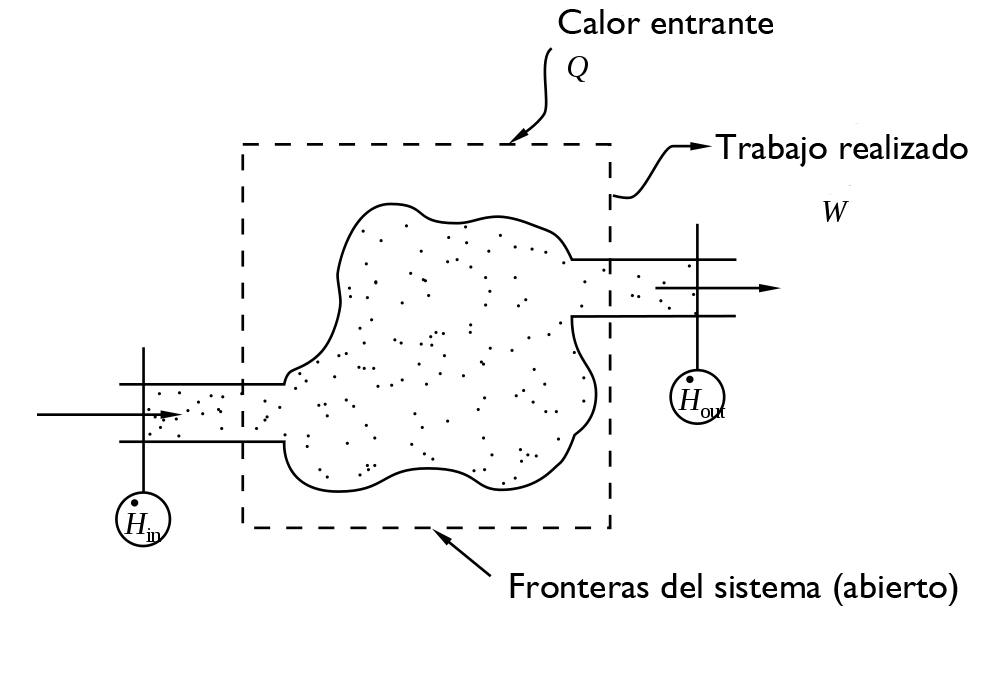
\includegraphics[width=0.60\textwidth]{Figure1.png}
	\caption{Ejemplo de sistema abierto}
\end{figure}

Considere un sistema como el que se muestra en la figura 1. El sistema recibe cierto calor $Q$ y realiza un trabajo $W$, pero también está sujeto a un flujo continuo de algún material que hace variar su masa además de que hace variar su energía interna.

Para realizar una descripción más adecuada de los sistemas abiertos es necesario definir el concepto de \textit{fase} y de \textit{sistema heterogéneo}.

La fase es la parte de un sistema, físicamente diferente, macroscópicamente homogénea y de composición fija o variable. Puede separarse mecánicamente del resto del sistema.

El sistema heterogéneo es aquel formado por dos o más fases entre las cuales hay fronteras.

\subsection{Formulación}
Dado que se define un sistema abierto como aquel que intercambia masa con sus alrededores entonces es razonable suponer que la ecuación de estado de este sistema esté en función del número de moles de cada componente del sistema (figura 2). Entonces

\[
	U = U(p, V, \eta_1, \cdots, \eta_r)
\]

\begin{figure}[h!]
	\centering
		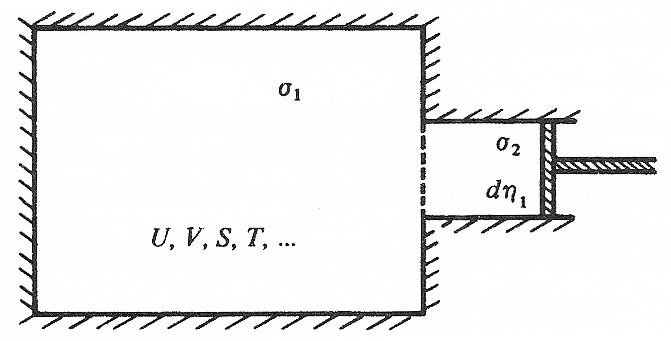
\includegraphics[width=0.60\textwidth]{Figure2.png}
	\caption{Dos sistemas termodinámicos}
\end{figure}

La diferencial $dU$ queda
\begin{equation}
	dU = \left ( \frac{\partial U}{\partial S} \right )_{V, \eta_i} dS + \left ( \frac{\partial U}{\partial V} \right )_{s, \eta_i} dV + \left ( \frac{\partial U}{\partial \eta_1} \right )_{V, S, \eta_{1 \neq r}} d \eta_1 + \cdots +  \left ( \frac{\partial U}{\partial \eta_r} \right )_{V, S, \eta_{i \neq r}} d \eta_r
\end{equation}

También, de la ecuación (2) se introducen las variables $X_i$ de las cuales depende la función $U$ definida anteriormente: $p, V, \eta_1, \cdots, \eta_r$. Sean $\mu_j$ los coeficientes correspondientes a los $\eta_j$.

\begin{equation}
	d U = T dS - p dV + \sum_j \mu_j d \eta_j
\end{equation}

entonces de las ecuaciones (3) y (4) se tiene
\[
	T = \left (\frac{\partial U}{\partial S}  \right )_{V, \eta_i}, \; \; p = - \left ( \frac{\partial U}{\partial V} \right )_{S, \eta_i}, \; \; \mu = \left ( \frac{\partial U}{\partial \eta_j} \right )_{V, S, \eta_{i \neq j}}
\]

Pero para que estas relaciones sean válidas es menester justificar primero que
\[
	U = U(p, V, \eta_1, \cdots, \eta_r)
\]

Para ello se tomará como hipótesis que la energía total de un sistema como el que se muestra en la figura 2 es la suma de las energias de cada una de las fases, es decir que cumple con la propiedad de aditividad.

Para explorar más esta idea se investigará cuál es el cambio de energía de este sistema al introducir $d \eta_i$ moles. Sean dos sistemas $\omega_1$ y $\omega_2$ con energías $U_1$ y $U_2$.

Por la hipótesis de la aditividad de la energía
\[
	U_{1+2} = U_1 + d U_2
\]

Sean
\[
	u_i = \frac{U_i}{\eta_i}, \; v_i = \frac{V_i}{\eta_i}, \; s_i = \frac{S_i}{\eta_i}
\]

la energía molar, volumen molar y entropía molar de la sustancia $i$ respectivamente.

Se introducirán los $d \eta_1$ moles al sistema $\omega_1$ que se muestra en la figura 2. Al hacer esto existe una contribución energética por introducir los $d \eta_1$, llámese $dU_2$ y existe otra contribución por el trabajo necesario para introducir los $d \eta_1$, que se llamará $dU'_2$.

Por la definición anterior
\[
	dU_2 = u_i d \eta_i
\]

Y la contribución energética $dU'_2$ es
\[
	dU'_2 = p dV = P_i v_i d \eta_i
\]

Entonces el cambio de energía será
\[
	dU = dU_2 + dU'_2 = (u_i + P_i v_i) d \eta_i
\]

Entonces para las $r$ sustancias que interactúan en este sistema
\[
	dU = \sum_{i=1}^r (u_i + P_i v_i) d \eta_i
\]

Hasta ahora sólo se consideró un sistema que no intercambia calor con sus alrededores ni realiza trabajo. Considerando estos términos se obtiene la primera ley de la termodinámica para sistemas abiertos.

\[
	dU = \delta Q + \delta W + \sum_{i=1}^r (u_i + P_i v_i) d \eta_i
\]

Para la descripción de la entropía en un sistema abierto considere que la entropía es una variable extensiva y por lo tanto aditiva. Anteriormente se había definido
\[
	s_i = \frac{S_i}{\eta_i}
\]

Por lo tanto
\[
	d S_2 = s_i d \eta_i
\]

El incremento de entropía al introducir los $d \eta_1$ moles es
\[
	d S_2 = \sum_{i=1}^r s_i d \eta_i
\]

Entonces
\[
	d S = \frac{\delta Q}{T} + \sum_{i=1}^r s_i d \eta_i
\]

que es la segunda ley de la termodinámica para sistemas abiertos.

De aquí se puede despejar el término $\delta Q$
\[
	\delta Q = T dS - \sum_{i=1}^r s_i d \eta_i
\]

y se sustituye en la primera ley de la termodinámica para sistemas abiertos
\[
	dU = T dS - \sum_{i=1}^r T s_i d \eta_i + \delta W +  \sum_{i=1}^r (u_i + P_i v_i) d \eta_i
\]

Considerando un sistema que sólo realiza trabajo $p dV$ queda
\[
	dU = T dS - p dV + \sum_{i=1}^r (u_i + P_i v_i - Ts_i) d \eta_i
\]

Comparándolo con la ecuación (4) la naturaleza del término $\mu$ queda clara
\[
	\mu = u_i + P_i v_i - T s_i
\]

Esto a su vez presenta semejanza con la energía libre de Gibbs descrita anteriormente. De hecho
\[
	\mu_i = \frac{G_i}{\eta_1}
\]

De manera que la $\mu_i$ es el potencial químico de la i-ésima componente.

\section{Conclusión}
Se han obtenido las expresiones equivalentes para la primera y segunda leyes de la termodinámica. Siendo
\[
	d U = T dS - p dV + \sum_j \mu_j d \eta_j
\]
la primera ley de la termodinámica,
\[
	d S = \frac{\delta Q}{T} + \sum_{i=1}^r s_i d \eta_i
\]
la segunda ley. También se ha obtenido una expresión capaz de definir el potencial químico
\[
	\mu_i = \frac{G_i}{\eta_i} = u_i + P_i v_i - T s_i
\]


\section{Bibliografía}
\renewcommand*{\refname}{}
\begin{thebibliography}{100}
\bibitem{Review} Review of Thermodynamics, James J. Kelly
\bibitem{Coling} Introducción a la termodinámica clásica, Leopoldo García-Colín Scherer. 4a edición. México. Trillas, 1990.
\bibitem{Abiertos} Introducción a la termodinámica de sistemas abiertos. Leopoldo García-Colín Scherer. El Colegio Nacional. México, 1981.
\end{thebibliography}

\end{document}